%----------------------------------------------------%
%       ANÁLISIS DE LAS TÉCNOLOGÍAS PROPUESTAS       %
%----------------------------------------------------%

\pagestyle{fancy}

\chapter{Análisis de las tecnologías propuestas}
\label{introduccion}

\section{Apache Cassandra}

a.\\

Apache Cassandra[12] es una base de datos distribuida desarrollada por DataStax bajo la licencia de Apache que trabaja con datos de tipo clave/valor.

El no tener ni un único punto de fallo le posibilita ofrecer una disponibilidad continua, además de otros servicios como la alta escalabilidad, alto rendimiento, seguridad y una simplicidad operacional que permite reducir el coste total de propiedad. Está siendo utilizada por muchas de las aplicaciones en negocios modernos, siendo la base de datos elegida por un cuarto de las empresas de la Fortune 100[].

Debido a la apuesta realizada a favor de Spark por parte de DataStax, esta empresa ha desarrollado un conector para enlazar Spark y Cassandra utilizando funciones de alto nivel de abstracción.

Será recomendable utilizar Cassandra si:
%
%•	se desea que la configuración, mantenimiento y el código sea sencillo.
%•	se necesitan velocidades muy altas en lecturas y escrituras aleatorias.
%•	no se necesitan múltiples índices secundarios
%•	existe alta flexibilidad en la estructura de los datos 
%•	se busca una escalabilidad masiva
%•	se busca alta disponibilidad

No será recomendable utilizar Cassandra si:

%•	se manejan datos relacionales
%•	hay transacciones de por medio
%•	se requiere autorización para acceder a datos
%•	se busca por columnas
%•	se necesita latencia baja

Como ya se ha apuntado anteriormente, Cassandra en una base de datos NoSQL distribuida que es instalada en todos los nodos del cluster. Aunque físicamente los datos estén repartidos en diferentes máquinas, ofrece la impresión de estar operando como una sola gracias a la capacidad de intercambiar los datos entre los diferentes nodos. Para lograr que todos ellos funcionen de manera coordinada, Cassandra utiliza un protocolo Gossip posibilitando que mediante paso de mensajes periódicamente se dé a conocer el estado de un nodo al resto de los nodos del cluster. Este protocolo es el que posibilita, entre otras cosas, que cada nodo pueda mantener actualizadas sus replicas.

Cassandra, como se acaba de mencionar, posibilita replicar los datos que se almacenan en la base de datos y acceder a ellos mediante un protocolo P2P. Un nodo posee una réplica para un cierto rango de datos y si un nodo falla, otro que tenga la réplica puede responderá a la petición sin tener que interrumpir el servicio. El número de réplicas que se quieren almacenar se especifica a la hora de crear el keyspace. Otro de los atributos que se debe especificar a la hora de crear un keyspace es la denominada Replica Placemente Startegy, la cual indica la forma en la que se reparten las repicas por el anillo.

homogeneridad de sus nodos

En cuanto a la estructura se refiere, un keyspace es un espacio de nombres para un conjunto de ColumFamily. Por lo general se utiliza uno por aplicación y es considerado el equivalente a una base de datos del modelo relacional. El ColumFamily, a su vez, es capaz de almacenar diferentes columnas, siendo el homologo de una tabla del modelo relacional. Para finalizar, una columna seria una estructura compuesta por clave, valor y timestamp.


Ilustración 5. Estructura de Cassandra

%Cabe mencionar que el almacenamiento de las columnas en a base de datos no es aleatoria. Cassandra almacena los datos dependiendo del primer atributo especificado en la clausula primary_key a la hora de crear el ColumFamily, guardando en el mismo nodo las columnas que comparten el valor de dicho atributo. Por ejemplo, si se especificarán las dos siguientes claves primarias:

%En ambos casos la clave primaria vendría a ser la misma, la combinación de los tres atributos que aparecen entre paréntesis. No obstante, Cassandra no almacenaría los datos de igual forma en ambos casos. En el primero, los datos con un mismo username serían almacenados en el mismo nodo o en nodos vecinos a este, mientras que en la segundo, los datos almacenados siguiendo ese criterio de proximidad serían los que coincidiesen en username e interaction_date.

Planificar esta distribución es vital a la hora de operar con los datos en Apache Spark. En el próximo apartado en la cual se hablará del funcionamiento de Apache Spark se volverá a hablar de esto explicando con más detalle las implicaciones que tiene.

Teorema Brewer

Arquitectura homogénea


Cassandra Query Lenguage

Apache Cassandra posee su propio lenguaje de consultas, el denominado CQL, Cassandra Query Lenguage, que se amolda a las características de esta base de datos. La sintaxis de CQL guarda una gran similitud con la de SQL lo cual facilita de forma notoria el salto que supone pasar de trabajar con bases de datos relacionales a distribuidos. 

Aún siendo sintácticamente  tan parecido a SQL, presenta ciertas restricciones debido a ser un lenguaje de consultas de una base de datos distribuida. Por ejemplo, no ofrece la posibilidad de realizar operaciones como JOIN y es totalmente necesario especificar todas los atributos que componen la clave primaria a la hora de realizar cualquier consulta de filtrado o de actualización en la tabla. La única operación que no cumple esta restricción es un select que contenga la clausula where, ya que, al definir la clave primaria Cassandra indexa de forma automática todos sus componente, posibilitando más tarde  hacer uso de ellos en este caso concreto.

Otra de las peculiaridades que presenta CQL es el hecho de ofrecer dos modos distintos de realizar un update. El primero de todos es el mencionado en el párrafo anterior. El segundo posibilita actualizar una columna realizando un insert repitiendo el valor de las claves primarias de una columna ya existente en la base de datos. Esta segunda forma es cómoda a la par de peligrosa porque Cassandra no notifica si una clave primaria ya existe en la base de datos o no, pudiendo un insert desencadenar en un update no deseado.  


\section{Apache Spark}

Apache Spark[9] es un proyecto open source de computación en clúster. Desde el principio fue diseñado para poder ejecutar algoritmos iterativos en memoria sin la necesidad de almacenar en disco los resultados intermedios generados durante el proceso. Esta peculiaridad permite que los procesamientos llevados a cabo con Spark puedan llegar a ser, en algunos casos concretos, 100 veces más rápidos que los de MapReduce[10].\\

A mediados de 2014, coincidiendo con el lanzamiento de la primera versión, alcanzó la cifra de 465 colaboradores, convirtiéndolo en el proyecto más activo entre los relacionados con el Big Data dentro de la Apache Software Fundation.\\

Apache Spark está compuesto por múltiples y variados componentes que pueden ser utilizados de forma conjunta.\\

\begin{figure}[h]
	\centering
	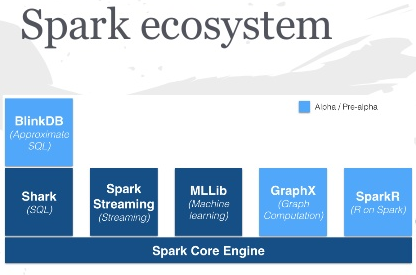
\includegraphics[width=0.5\textwidth]{Ilustraciones/spark_ecosystem.png}
	\caption{Ecosistema Spark}
	\label{fig:ipanel}
\end{figure}

La base del proyecto es el denominado Spark Core. Proporciona envío distribuido de tareas, planificación y funciones básicas de entrada salida. La abstracción fundamental de programación se llama Resilient Distributed Datasets (RDD)[11], una colección lógica de datos particionados a través de las máquinas que se expone mediante una API integrada en lenguajes como Java, Python y Scala.\\

\subsection{Funcionamiento}

Para el funcionamiento de Spark, es condición sine qua non que los nodos de la infraestructura tengan acceso a la totalidad de los datos que se desea tratar. Ello implica que para procesar un fichero de 50GB, cada nodo tendría que poseer una copia del mismo almacenado en su disco. Esta praxis es inviable, ya que más allá de los problemas de consistencia que generaría, para nada es eficiente ocupar la memoria de todos los nodos con información redundante y procesar el fichero entero cuando en realidad se va a hacer uso de una pequeña porción de dichos datos en cada ejecución.\\

Las bases de datos distribuidas como Cassandra solventan los problemas anteriormente mencionados. Se encargan de distribuir los datos entre diferentes nodos del clúster, ofrecen la posibilidad de acceder a ellos desde cualquier punto y mantienen la consistencia de los mismos a cambio de sufrir una pequeña latencia en el caso de requerir información almacenada en otro nodo de la infraestructura.\\ 

Al ejecutar una aplicación que opera con Spark, un componente denominado driver es lanzado. Debido a la necesidad de obtener recursos (CPU y memoria) para llevar a cabo la computación que se le ha encomendado, se comunica con un nodo del clúster que, mediante especificación previa, adopta el rol de maestro. Éste pregunta a todos los nodos que conforman la infraestructura sobre la cantidad de recursos disponibles que poseen y así asignarles los executors correspondiente. Las máquinas que alojen al menos un executor pasan a denominarse worker y a partir de este momento, cada executor podrá comunicarse directamente con el Driver para poder recibir las tareas que éste le envíe.\\

Un executor es una unidad de trabajo que se encarga de computar las tareas que le encomienda el driver. El número de executors que puede albergar cada worker está directamente relacionado con el número de procesadores que este posee. De la misma forma, es posible repartir la memoria RAM que dispone el nodo worker entre varios executors. Spark permite modificar ambos parámetros programáticamente permitiendo así poder amoldarse a las particularidades de cada ejecución.\\

Para transferir el código del programa, residente en la máquina del driver, éste adopta  el rol de servidor e intenta enviar dicho código a los workers. Si el fichero JAR que contiene el código ha sido recibido correctamente por sus destinatarios, estos responden mediante un ACK y en caso contrario, se vuelve a intentar el envío un número determinado de veces. Una vez llegado al máximo de reintentos, el worker que no haya enviado el ACK es considerado como caído, quedando los executors que albergaba fuera del posterior reparto de tareas.\\

\begin{figure}[h]
	\centering
	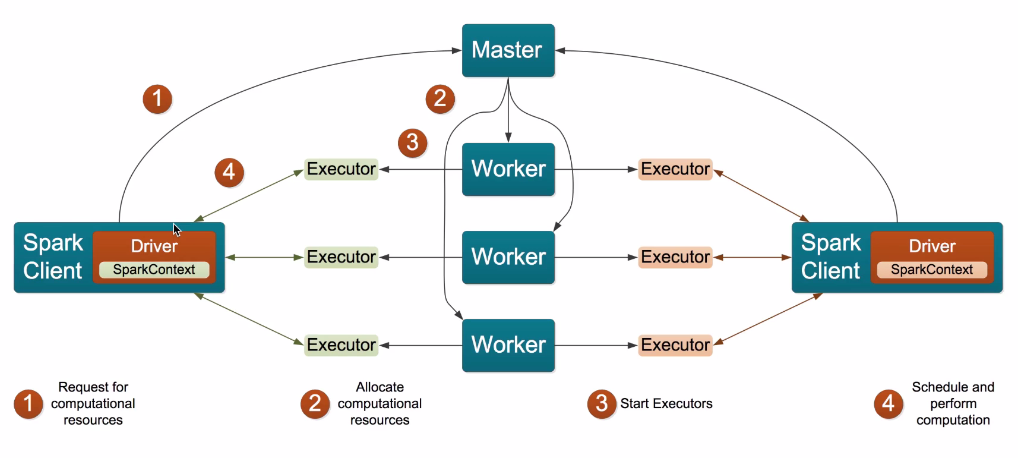
\includegraphics[width=1\textwidth]{Ilustraciones/spark_architecture.png}
	\caption{Arquitectura Spark}
	\label{fig:spark_architecture}
\end{figure}

A la hora de realizar operaciones en Spark, el objeto estrella es el denominado Resilient Distributed Datasets (RDD)[11]. Se trata de una abstracción que mediante diferentes APIs disponibles para Java, Scala y Python permite manipular datos distribuidos por los diferentes nodos del clúster como si estuvieran almacenados de forma local. Este objeto es inmutable, lo cual implica que una vez creado no se le pueden añadir nuevos elementos o eliminar los existentes, solo aplicar transformaciones y acciones sobre el.\\

Las operaciones que se pueden realizar sobre las RDD se agrupan, tal y como se ha adelantado antes, por transformaciones y acciones. Las primeras transforman un RDD en otro según el criterio indicado y las segundas realizan modificaciones sobre los datos almacenados en dichas RDD. Cabe destacar que las transformaciones en Spark son operaciones "lazy", lo cual implica que en realidad cada nodo memoriza la secuencia de transformaciones que ha de realizar y los procesa cuando una acción es ejecutada.\\

Una vez terminada la primera fase en la que los executor son creados y enlazados con el driver, éste último empieza a analizar la estructura del código y genera un grafo DAG (Directed Acyclic Graph) con las operaciones que se realizan sobre la RDD. Partiendo de ese grafo genera un job por cada operación de tipo acción que encuentra y dentro de cada job separa la ejecución en diferentes stages según las dependencias que existan entre operaciones. Por último, cada stage es dividido por defecto en unidades de 64MB y a cada unidad resultante se denomina task, el cual es enviado a un executor para ser procesado. El tamaño de cada task puede ser modificado programáticamente, pudiendo de esa forma manipular el número de task que un executor deba ejecutar.\\

\begin{figure}[h]
	\centering
	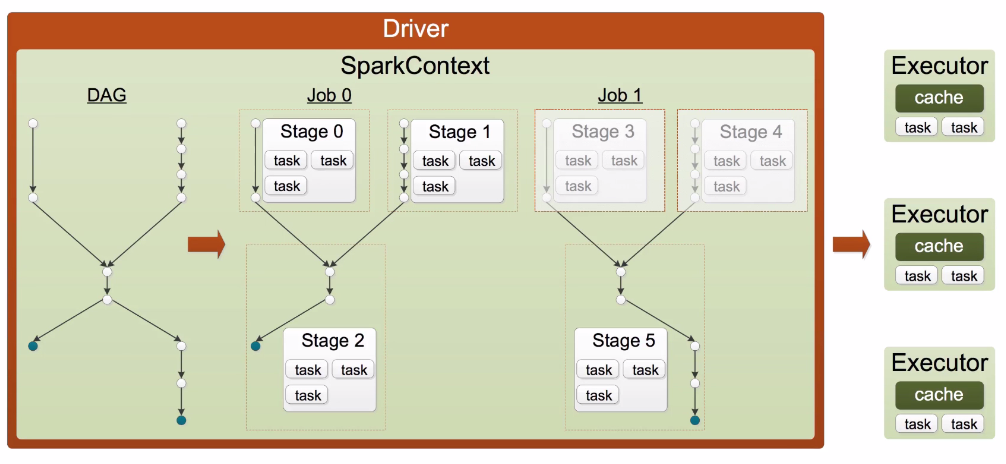
\includegraphics[width=1\textwidth]{Ilustraciones/spark_task_creation.png}
	\caption{Arquitectura Spark}
	\label{fig:spark_task_creation}
\end{figure}

El Driver, una vez habiendo recibido los resultados de todas los task que ha repartido, enviará un mensaje a los executors indicando que el procesamiento ha sido finalizado y calculará el resultado final ofreciendo la posibilidad de, por ejemplo, almacenarlo en una base de datos distribuida como Cassandra.\\






